Eine Zufallsvariable $X$ ist auf dem Intervall $[0,\pi]$ so verteilt,
dass die Wahrscheinlichkeitsdichte
\[
\varphi_X(x)
=
\begin{cases}
0&\qquad x < 0\\
a(1-\sin x)&\qquad 0\le x \le \pi\\
0&\qquad x > \pi
\end{cases}
\]
ist wie in dem folgenden Graphen:
\begin{center}
\definecolor{darkred}{rgb}{0.8,0,0}
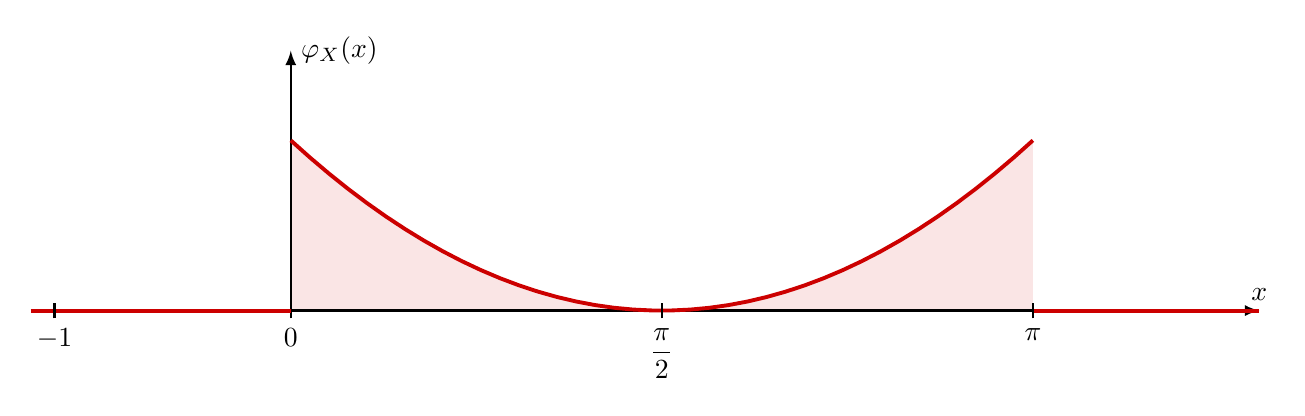
\begin{tikzpicture}[>=latex,thick]
\def\h{3}
\fill[color=darkred!10]
	plot[domain=0:3.1415,samples=40]
		({\x*\h},{(\x-3.14159/2)*(\x-3.14159/2)/(3.14159-2)})
	-- ({3.14159*\h},0) -- (0,0) -- cycle;
\draw[->] ({-1.1*\h},0) -- ({4.1*\h},0) coordinate[label={$x$}];
\draw[->] (0,-0.1) -- (0,{1.1*\h}) coordinate[label={right:$\varphi_X(x)$}];
\draw[color=darkred,line width=1.4pt] ({-1.1*\h},0) -- (0,0);
\draw[color=darkred,line width=1.4pt]
	plot[domain=0:3.1415,samples=40]
		({\x*\h},{(\x-3.14159/2)*(\x-3.14159/2)/(3.14159-2)});
\draw[color=darkred,line width=1.4pt] ({3.14159*\h},0) -- ({4.1*\h},0);
\foreach \x in {-1,{3.14159/2},3.14159}{
	\draw ({\x*\h},-0.1) -- ({\x*\h},0.1);
}
\node at ({-1*\h},-0.1) [below] {$-1$};
\node at (0,-0.1) [below] {$0$};
\node at ({0.5*3.14159*\h},-0.1) [below] {$\displaystyle\frac{\pi}{2}$};
\node at ({3.14156*\h},-0.1) [below] {$\pi$};
\end{tikzpicture}
%\includeagraphics[]{graph-1.pdf}
\end{center}
\begin{teilaufgaben}
\item
Wie muss man $a$ wählen, damit diese Funktion tatsächlich 
eine Wahrscheinlichkeitsdichte ist?
\item
Berechnen Sie $E(X)$ und $\operatorname{var}(X)$.
\end{teilaufgaben}

\thema{Wahrscheinlichkeitsdichte}
\thema{Verteilungsfunktion}
\thema{Erwartungswert}
\thema{Varianz}

\begin{loesung}
\begin{teilaufgaben}
\item Die Konstante $a$ muss so gewählt werden, dass das Integral von
$\varphi_X$ über $\mathbb R$ den Wert 1 hat:
\[
\int_{-\infty}^{\infty}\varphi_X(x)\,dx
=
\int_0^\pi a(1-\sin x)\,dx
=
a[x+\cos x]_0^\pi
=
a(\pi - 1 - 0 - 1) = a(\pi-2)
\]
es folgt
\[
a=\frac1{\pi -2}=0.87597.
\]
\item
Für den Erwartungswert $E(X)$ müssen wir $x\varphi_X(x)$ integrieren:
\begin{align*}
E(X)
&=
\int_{-\infty}^\infty x\varphi_X(x)\,dx
=
\frac1{\pi-2}\int_0^\pi x(1-\sin x)\,dx
=
\frac1{\pi - 2} \biggl[\frac{x^2}{2}-\sin x + x\cos x\biggr]_0^\pi
\\
&=
\frac1{\pi - 2}\biggl(\frac{\pi^2}{2} +\pi\cos\pi\biggr)
=
\frac{\pi^2-2\pi}{2(\pi-2)}=\frac{\pi}{2} = 1.57079,
\end{align*}
dies ist natürlich nicht überraschend, da die Verteilung um diesen
Punkt symmetrisch ist.

Für die Varianz brauchen wir $E(X^2)$:
\begin{align*}
E(X^2)
&=
\int_{-\infty}^\infty x^2\varphi_X(x)\,dx
=
\frac1{\pi-2}\int_0^\pi x^2(1-\sin x)\,dx
=
\frac1{\pi-2}\biggl[
\frac{x^3}{3}-2x\sin x+(x^2-2)\cos x
\biggr]_0^\pi
\\
&=
\frac{\pi^3-3\pi^2+12}{3(\pi-2)}
=
3.9119
\\
\operatorname{var}(X)
&=
E(X^2)-E(X)^2
=
\frac{\pi^3-3\pi^2+12}{3\pi - 6}
-
\frac{\pi^2}{4}
=
\frac {\pi^3-6\pi^2+48}{12\pi-24}
=
1.44452.
\end{align*}
Die Resultate sind in Abbildung~\ref{50000030:graphplus} visualisiert
\begin{figure}
\centering
\definecolor{darkred}{rgb}{0.8,0,0}
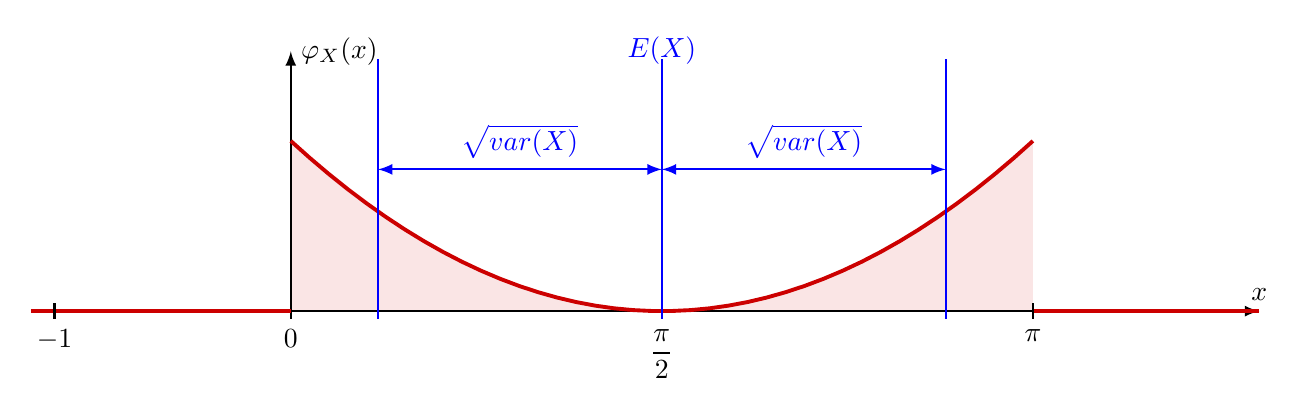
\begin{tikzpicture}[>=latex,thick]
\def\h{3}
\fill[color=darkred!10]
	plot[domain=0:3.1415,samples=40]
		({\x*\h},{(\x-3.14159/2)*(\x-3.14159/2)/(3.14159-2)})
	-- ({3.14159*\h},0) -- (0,0) -- cycle;
\draw[->] ({-1.1*\h},0) -- ({4.1*\h},0) coordinate[label={$x$}];
\draw[->] (0,-0.1) -- (0,{1.1*\h}) coordinate[label={right:$\varphi_X(x)$}];
\draw[color=darkred,line width=1.4pt] ({-1.1*\h},0) -- (0,0);
\draw[color=darkred,line width=1.4pt]
	plot[domain=0:3.1415,samples=40]
		({\x*\h},{(\x-3.14159/2)*(\x-3.14159/2)/(3.14159-2)});
\draw[color=darkred,line width=1.4pt] ({3.14159*\h},0) -- ({4.1*\h},0);
\foreach \x in {-1,{3.14159/2},3.14159}{
	\draw ({\x*\h},-0.1) -- ({\x*\h},0.1);
}
\node at ({-1*\h},-0.1) [below] {$-1$};
\node at (0,-0.1) [below] {$0$};
\node at ({0.5*3.14159*\h},-0.1) [below] {$\displaystyle\frac{\pi}{2}$};
\node at ({3.14156*\h},-0.1) [below] {$\pi$};
\draw[color=blue] ({0.5*3.14159*\h},-0.1) -- ++(0,{1.1*\h});
\draw[color=blue] ({(0.5*3.14159-sqrt(1.44452))*\h},-0.1) -- ++(0,{1.1*\h});
\draw[color=blue] ({(0.5*3.14159+sqrt(1.44452))*\h},-0.1) -- ++(0,{1.1*\h});
\draw[<->,color=blue] ({0.5*3.14159*\h},{0.6*\h}) -- ++({-sqrt(1.44452)*\h},0);
\draw[<->,color=blue] ({0.5*3.14159*\h},{0.6*\h}) -- ++({sqrt(1.44452)*\h},0);
\node[color=blue] at ({0.5*(3.14159-sqrt(1.4452))*\h},{0.6*\h})
	[above] {$\sqrt{\operatorname{var}(X)}$};
\node[color=blue] at ({0.5*(3.14159+sqrt(1.4452))*\h},{0.6*\h})
	[above] {$\sqrt{\operatorname{var}(X)}$};
\node[color=blue] at ({0.5*3.14159*\h},{\h}) [above] {$E(X)$};
\end{tikzpicture}
%\includeagraphics[]{graph-2.pdf}
\caption{Wahrscheinlichkeitsdichte $\varphi_X(x)$ aus Aufgabe~\ref{50000030}
mit $E(X)$ und Varianz.
\label{50000030:graphplus}}
\end{figure}
\qedhere
\end{teilaufgaben}
\end{loesung}

\begin{bewertung}
Normierungsbedingung für die Bestimmung von $a$ ({\bf N}) 1 Punkt,
Wert von $a$ ({\bf A}) 1 Punkt,
Formeln für $E(X)$ und $E(X^2)$ ({\bf F}) 1 Punkt,
Erwartungswert ({\bf E}) 1 Punkt,
Erwartungswert $E(X^2)$ ({\bf X}) 1 Punkt,
Varianz ({\bf V}) 1 Punkt.
\end{bewertung}

